
                \begin{figure}
                    \centering
                    \begin{tikzpicture}
                        \pgfplotsset{%
                            width=1\textwidth,
                            height=0.5\textheight
                        }
                        \begin{axis}[
                            xlabel={Start battery level},
                            ylabel={Average dynamic energy (watt)},
                            ymin=0,ymax=20,
                        ]
                        
                            \addplot [mark=none, ultra thick, red]  coordinates {
                            (40, 9.057649533891459)(45, 9.097512579496243)(50, 9.133047352741833)(55, 9.094676667014697)(60, 9.092498304923305)(65, 9.171510701094066)(70, 9.177326681813389)(75, 9.110286025516734)(80, 8.9217459766221)
                            };
                            \addlegendentry{Surface4Pro - IntelPowerGadget}
                            
                            \addplot [mark=none, ultra thick, blue]  coordinates {
                            (40, 9.184044279462524)(45, 9.17760165750797)(50, 9.185078019225433)(55, 9.185394897691006)(60, 9.223123393410514)(65, 9.208160534605785)(70, 9.216409513651284)(75, 9.182619156358658)(80, 8.88296766865553)
                            };
                            \addlegendentry{Surface4Pro - HardwareMonitor}
                            
                            \addplot [mark=none, ultra thick, orange]  coordinates {
                            (50, 6.894114910098497)(55, 6.911696910459913)(60, 6.913009542945647)(65, 6.913413915769665)(70, 6.907049697911252)(75, 6.869638141000093)(80, 6.766853468931586)
                            };
                            \addlegendentry{Surface4Pro - RAPL}
                            
                            \addplot [mark=none, dashdotted, red]  coordinates {
                            (40, 2.661306204402436)(45, 2.631057764991513)(50, 2.6720505655991555)(55, 2.6187618885181587)(60, 2.6284510136688435)(65, 2.6895115018894193)(70, 2.664863357463519)(75, 2.692526207526449)(80, 2.7261483389248236)
                            };
                            \addlegendentry{SurfaceBook - IntelPowerGadget}
                            
                            \addplot [mark=none, dashdotted, blue]  coordinates {
                            (40, 4.377885120927457)(45, 4.37295929970067)(50, 4.397655430510698)(55, 4.382934211865668)(60, 4.394984027902462)(65, 4.3876141345038935)(70, 4.3934458191290044)(75, 4.3808183016906375)(80, 4.429594212848234)
                            };
                            \addlegendentry{SurfaceBook - HardwareMonitor}
                            
                            \addplot [mark=none, dashdotted, orange]  coordinates {
                            (40, 4.824050337037943)(45, 4.8158335396402)(50, 4.830043303870358)(55, 4.820128973088121)(60, 4.823079295850169)(65, 4.814171143136699)(70, 4.820604111528336)(75, 4.845715237193803)(80, 4.844606185367628)
                            };
                            \addlegendentry{SurfaceBook - RAPL}
                            
                        \end{axis}
                    \end{tikzpicture} 
                \caption{A graph illustrating the energy consumption of Cores for test case Nbody with regards to the battey level of the DUT (without outliers)} \label{fig:Nbody_Cores_charge}
                \end{figure}
                